%% abtex2-modelo-trabalho-academico.tex, v-1.9.2 laurocesar
%% Copyright 2012-2014 by abnTeX2 group at http://abntex2.googlecode.com/ 
%%
%% This work may be distributed and/or modified under the
%% conditions of the LaTeX Project Public License, either version 1.3
%% of this license or (at your option) any later version.
%% The latest version of this license is in
%%   http://www.latex-project.org/lppl.txt
%% and version 1.3 or later is part of all distributions of LaTeX
%% version 2005/12/01 or later.
%%
%% This work has the LPPL maintenance status `maintained'.
%% 
%% The Current Maintainer of this work is the abnTeX2 team, led
%% by Lauro César Araujo. Further information are available on 
%% http://abntex2.googlecode.com/
%%
%% This work consists of the files abntex2-modelo-trabalho-academico.tex,
%% abntex2-modelo-include-comandos and abntex2-modelo-references.bib
%%

% ------------------------------------------------------------------------
% ------------------------------------------------------------------------
% abnTeX2: Modelo de Trabalho Academico (tese de doutorado, dissertacao de
% mestrado e trabalhos monograficos em geral) em conformidade com 
% ABNT NBR 14724:2011: Informacao e documentacao - Trabalhos academicos -
% Apresentacao
% ------------------------------------------------------------------------
% ------------------------------------------------------------------------

\documentclass[
	% -- opções da classe memoir --
	12pt,				% tamanho da fonte
	openright,			% capítulos começam em pág ímpar (insere página vazia caso preciso)
	twoside,			% para impressão em verso e anverso. Oposto a oneside
	a4paper,			% tamanho do papel. 
	% -- opções da classe abntex2 --
	%chapter=TITLE,		% títulos de capítulos convertidos em letras maiúsculas
	%section=TITLE,		% títulos de seções convertidos em letras maiúsculas
	%subsection=TITLE,	% títulos de subseções convertidos em letras maiúsculas
	%subsubsection=TITLE,% títulos de subsubseções convertidos em letras maiúsculas
	% -- opções do pacote babel --
	english,			% idioma adicional para hifenização
	french,				% idioma adicional para hifenização
	spanish,			% idioma adicional para hifenização
	brazil				% o último idioma é o principal do documento
	]{abntex2}

% ---
% Pacotes básicos 
% ---
\usepackage{lmodern}			% Usa a fonte Latin Modern			
\usepackage[T1]{fontenc}		% Selecao de codigos de fonte.
\usepackage[utf8]{inputenc}		% Codificacao do documento (conversão automática dos acentos)
\usepackage{lastpage}			% Usado pela Ficha catalográfica
\usepackage{indentfirst}		% Indenta o primeiro parágrafo de cada seção.
\usepackage{color}				% Controle das cores
\usepackage{graphicx}			% Inclusão de gráficos
\usepackage{microtype} 			% para melhorias de justificação
\usepackage[final]{pdfpages}
\usepackage{url}
\usepackage{float}
\usepackage{amsmath}
\usepackage{cleveref}
\usepackage{pgfplots}
\usepackage{amsfonts}
\usepackage{amsmath}
\usepackage{tikz}
\usetikzlibrary{matrix, positioning}

\DeclareMathOperator{\logsumexp}{logsumexp}
\pgfmathdeclarefunction{sumexp}{3}{%
  \begingroup%
  \pgfkeys{/pgf/fpu}% "/pgf/fpu/output format=fixed" removed
  \pgfmathsetmacro{\myx}{#1}%
  \pgfmathtruncatemacro{\myxmin}{#2}%
  \pgfmathtruncatemacro{\myxmax}{#3}%
  \pgfmathsetmacro{\mysum}{0}%
  \pgfplotsforeachungrouped\XX in {\myxmin,...,\myxmax}%
    {\pgfmathsetmacro{\mysum}{\mysum+exp(\XX)}}%
  \pgfmathparse{\mysum+exp(#1)}%
  \pgfmathfloattofixed\pgfmathresult%  added
  \pgfmathsmuggle\pgfmathresult\endgroup%
}

\crefname{figure}{Figura}{Figuras}
% ---
		
% ---
% Pacotes adicionais, usados apenas no âmbito do Modelo Canônico do abnteX2
% ---
\usepackage{lipsum}				% para geração de dummy text
% ---

% ---
% Pacotes de citações
% ---
\usepackage[brazilian,hyperpageref]{backref}	 % Paginas com as citações na bibl
\usepackage[alf]{abntex2cite}	% Citações padrão ABNT

% --- 
% CONFIGURAÇÕES DE PACOTES
% --- 

% ---
% Configurações do pacote backref
% Usado sem a opção hyperpageref de backref
\renewcommand{\backrefpagesname}{Citado na(s) página(s):~}
% Texto padrão antes do número das páginas
\renewcommand{\backref}{}
% Define os textos da citação
\renewcommand*{\backrefalt}[4]{
	\ifcase #1 %
		Nenhuma citação no texto.%
	\or
		Citado na página #2.%
	\else
		Citado #1 vezes nas páginas #2.%
	\fi}%
% ---

% ---
% Informações de dados para CAPA e FOLHA DE ROSTO
% ---
\titulo{Geração procedural de mapas de ilhas 2d com biomas através de técnicas de segmentação de imagem}
\autor{Lucas da Silva dos Santos\\Matheus Zanivan Andrade\\ Rafael Nascimento Lourenço}
\local{São Paulo - Brasil}
\data{2023}
\orientador{Lauro César Araujo}
\coorientador{Equipe \abnTeX}
\instituicao{%
  Senac: Serviço Nacional de Aprendizagem Comercial
  \par
  Bacharelado em ciência da computação
}
\tipotrabalho{Trabalho de Conclusão de Curso (TCC)}
% O preambulo deve conter o tipo do trabalho, o objetivo, 
% o nome da instituição e a área de concentração 
\preambulo{Modelo canônico de trabalho monográfico acadêmico em conformidade com
as normas ABNT apresentado à comunidade de usuários \LaTeX.}
% ---


% ---
% Configurações de aparência do PDF final

% alterando o aspecto da cor azul
\definecolor{blue}{RGB}{41,5,195}

% informações do PDF
\makeatletter
\hypersetup{
     	%pagebackref=true,
		pdftitle={\@title}, 
		pdfauthor={\@author},
    	pdfsubject={\imprimirpreambulo},
	    pdfcreator={LaTeX with abnTeX2},
		pdfkeywords={abnt}{latex}{abntex}{abntex2}{trabalho acadêmico}, 
		colorlinks=true,       		% false: boxed links; true: colored links
    	linkcolor=blue,          	% color of internal links
    	citecolor=blue,        		% color of links to bibliography
    	filecolor=magenta,      		% color of file links
		urlcolor=blue,
		bookmarksdepth=4
}
\makeatother
% --- 

% --- 
% Espaçamentos entre linhas e parágrafos 
% --- 

% O tamanho do parágrafo é dado por:
\setlength{\parindent}{1.3cm}

% Controle do espaçamento entre um parágrafo e outro:
\setlength{\parskip}{0.2cm}  % tente também \onelineskip

% ---
% compila o indice
% ---
\makeindex
% ---

% ----
% Início do documento
% ----
\begin{document}

% Retira espaço extra obsoleto entre as frases.
\frenchspacing 

% ----------------------------------------------------------
% ELEMENTOS PRÉ-TEXTUAIS
% ----------------------------------------------------------
% \pretextual

% ---
% Capa
% ---
\imprimircapa
% ---

% ---
% Folha de rosto
% (o * indica que haverá a ficha bibliográfica)
% ---
\imprimirfolhaderosto*
% ---

% ---
% Inserir a ficha bibliografica
% ---
% Isto é um exemplo de Ficha Catalográfica, ou ``Dados internacionais de
% catalogação-na-publicação''. Você pode utilizar este modelo como referência. 
% Porém, provavelmente a biblioteca da sua universidade lhe fornecerá um PDF
% com a ficha catalográfica definitiva após a defesa do trabalho. Quando estiver
% com o documento, salve-o como PDF no diretório do seu projeto e substitua todo
% o conteúdo de implementação deste arquivo pelo comando abaixo:
%
\begin{fichacatalografica}
    \includepdf{ficha.pdf}
\end{fichacatalografica}
% ---

% ---
% Inserir errata
% ---
% \begin{errata}
% Elemento opcional da \citeonline[4.2.1.2]{NBR14724:2011}. Exemplo:

% \vspace{\onelineskip}

% FERRIGNO, C. R. A. \textbf{Tratamento de neoplasias ósseas apendiculares com
% reimplantação de enxerto ósseo autólogo autoclavado associado ao plasma
% rico em plaquetas}: estudo crítico na cirurgia de preservação de membro em
% cães. 2011. 128 f. Tese (Livre-Docência) - Faculdade de Medicina Veterinária e
% Zootecnia, Universidade de São Paulo, São Paulo, 2011.

% \begin{table}[htb]
% \center
% \footnotesize
% \begin{tabular}{|p{1.4cm}|p{1cm}|p{3cm}|p{3cm}|}
%   \hline
%    \textbf{Folha} & \textbf{Linha}  & \textbf{Onde se lê}  & \textbf{Leia-se}  \\
%     \hline
%     1 & 10 & auto-conclavo & autoconclavo\\
%    \hline
% \end{tabular}
% \end{table}

% \end{errata}
% ---

% ---
% Inserir folha de aprovação
% ---

% Isto é um exemplo de Folha de aprovação, elemento obrigatório da NBR
% 14724/2011 (seção 4.2.1.3). Você pode utilizar este modelo até a aprovação
% do trabalho. Após isso, substitua todo o conteúdo deste arquivo por uma
% imagem da página assinada pela banca com o comando abaixo:
%
% \includepdf{folhadeaprovacao_final.pdf}
%
\begin{folhadeaprovacao}

  \begin{center}
    {\ABNTEXchapterfont\large\imprimirautor}

    \vspace*{\fill}\vspace*{\fill}
    \begin{center}
      \ABNTEXchapterfont\bfseries\Large\imprimirtitulo
    \end{center}
    \vspace*{\fill}
    
    \hspace{.45\textwidth}
    \begin{minipage}{.5\textwidth}
        \imprimirpreambulo
    \end{minipage}%
    \vspace*{\fill}
   \end{center}
        
%    Trabalho aprovado. \imprimirlocal, 24 de novembro de 2012:

   \assinatura{\textbf{\imprimirorientador} \\ Orientador} 
   \assinatura{\textbf{Professor} \\ Convidado 1}
   \assinatura{\textbf{Professor} \\ Convidado 2}
   %\assinatura{\textbf{Professor} \\ Convidado 3}
   %\assinatura{\textbf{Professor} \\ Convidado 4}
      
   \begin{center}
    \vspace*{0.5cm}
    {\large\imprimirlocal}
    \par
    {\large\imprimirdata}
    \vspace*{1cm}
  \end{center}
  
\end{folhadeaprovacao}
% ---

% ---
% Dedicatória
% ---
\begin{dedicatoria}
   \vspace*{\fill}
   \centering
   \noindent
   \textit{ Este trabalho é dedicado às crianças adultas que,\\
   quando pequenas, sonharam em se tornar cientistas.} \vspace*{\fill}
\end{dedicatoria}
% ---

% ---
% Agradecimentos
% ---
\begin{agradecimentos}
Os agradecimentos principais são direcionados à Gerald Weber, Miguel Frasson,
Leslie H. Watter, Bruno Parente Lima, Flávio de Vasconcellos Corrêa, Otavio Real
Salvador, Renato Machnievscz\footnote{Os nomes dos integrantes do primeiro
projeto abn\TeX\ foram extraídos de
\url{http://codigolivre.org.br/projects/abntex/}} e todos aqueles que
contribuíram para que a produção de trabalhos acadêmicos conforme
as normas ABNT com \LaTeX\ fosse possível.

Agradecimentos especiais são direcionados ao Centro de Pesquisa em Arquitetura
da Informação\footnote{\url{http://www.cpai.unb.br/}} da Universidade de
Brasília (CPAI), ao grupo de usuários
\emph{latex-br}\footnote{\url{http://groups.google.com/group/latex-br}} e aos
novos voluntários do grupo
\emph{\abnTeX}\footnote{\url{http://groups.google.com/group/abntex2} e
\url{http://abntex2.googlecode.com/}}~que contribuíram e que ainda
contribuirão para a evolução do \abnTeX.

\end{agradecimentos}
% ---

% ---
% Epígrafe
% ---
\begin{epigrafe}
    \vspace*{\fill}
	\begin{flushright}
		\textit{``Não vos amoldeis às estruturas deste mundo, \\
		mas transformai-vos pela renovação da mente, \\
		a fim de distinguir qual é a vontade de Deus: \\
		o que é bom, o que Lhe é agradável, o que é perfeito.\\
		(Bíblia Sagrada, Romanos 12, 2)}
	\end{flushright}
\end{epigrafe}
% ---

% ---
% RESUMOS
% ---

% resumo em português
% \setlength{\absparsep}{18pt} % ajusta o espaçamento dos parágrafos do resumo
% \begin{resumo}
%  Segundo a \citeonline[3.1-3.2]{NBR6028:2003}, o resumo deve ressaltar o
%  objetivo, o método, os resultados e as conclusões do documento. A ordem e a extensão
%  destes itens dependem do tipo de resumo (informativo ou indicativo) e do
%  tratamento que cada item recebe no documento original. O resumo deve ser
%  precedido da referência do documento, com exceção do resumo inserido no
%  próprio documento. (\ldots) As palavras-chave devem figurar logo abaixo do
%  resumo, antecedidas da expressão Palavras-chave:, separadas entre si por
%  ponto e finalizadas também por ponto.

%  \textbf{Palavras-chaves}: latex. abntex. editoração de texto.
% \end{resumo}

% resumo em inglês
% \begin{resumo}[Abstract]
%  \begin{otherlanguage*}{english}
%    This is the english abstract.

%    \vspace{\onelineskip}
 
%    \noindent 
%    \textbf{Key-words}: latex. abntex. text editoration.
%  \end{otherlanguage*}
% \end{resumo}
% ---

% ---
% inserir lista de ilustrações
% ---
% \pdfbookmark[0]{\listfigurename}{lof}
% \listoffigures*
% \cleardoublepage
% ---

% ---
% inserir lista de tabelas
% ---
% \pdfbookmark[0]{\listtablename}{lot}
% \listoftables*
% \cleardoublepage
% ---

% ---
% inserir lista de abreviaturas e siglas
% ---
% \begin{siglas}
%   \item[ABNT] Associação Brasileira de Normas Técnicas
%   \item[abnTeX] ABsurdas Normas para TeX
% \end{siglas}
% ---

% ---
% inserir lista de símbolos
% ---
% \begin{simbolos}
%   \item[$ \Gamma $] Letra grega Gama
%   \item[$ \Lambda $] Lambda
%   \item[$ \zeta $] Letra grega minúscula zeta
%   \item[$ \in $] Pertence
% \end{simbolos}
% ---

% ---
% inserir o sumario
% ---
\pdfbookmark[0]{\contentsname}{toc}
\tableofcontents*
\cleardoublepage
% ---



% ----------------------------------------------------------
% ELEMENTOS TEXTUAIS
% ----------------------------------------------------------
\textual

% ----------------------------------------------------------
% Introdução (exemplo de capítulo sem numeração, mas presente no Sumário)
% ----------------------------------------------------------
\chapter{Introdução}
% ----------------------------------------------------------

\section{Contexto}

A indústria de jogos digitais cresce mais a cada dia, segundo a consultora Newzoo \space\cite{quanto_games_vao_movimentar} essa indústria tende a ultrapassar em 2023 os US\$ 200 bilhões (aproximadamente R\$ 1 trilhão). Novos jogos são produzidos e publicados diariamente e somente na plataforma digital Steam, foram publicados 10.963 novos títulos em 2022\space
\cite{numero_de_jogos_publicados_na_steam}.

Ademais, as empresas de desenvolvimento de jogos continuam a trabalhar incessantemente para atender a uma demanda de mercado que cresceu 2,5\% no Brasil em 2022 
\space
\cite{pesquisa_games_brasil}. O custo de produção de jogos varia bastante, dependendo do tamanho e da complexidade do projeto, \emph{e.g.}, a empresa Rockstar Games revelou que o jogo \"Grand Theft Auto V\" custou cerca de 265 milhões de dólares para ser produzido e comercializado \space
\cite{gta_quanto_custou}.

Outro cenário que está crescendo muito nos últimos anos é o da inteligência artificial afirma \citeonline{Valente_2020} que no Brasil mais que dobrou o número contratações de desenvolvedores da área de 2015 até 2020. De acordo com \apud{johnson2023}{briggs2023} um relatório recente relata que 300 milhões de empregos podem ser afetados pela IA \emph{i.e.} 18\% ofício global pode ser automatizado. Outrossim \citeonline{europarl2020} diz que o tópico de inteligência artificial é uma prioridade para União Europeia por ser considerada primordial para transformação digital da sociedade.  Do mesmo modo, "Bill Gates, um dos fundadores da Microsoft — uma das maiores empresas de tecnologia —, diz que o desenvolvimento da inteligência artificial (IA) é o avanço tecnológico mais importante em décadas"\space
\cite{inteligencia_artificial_e_avanco_bbc}.


\section{Justificativa}

O mapa é um elemento que se destaca em jogos digitais e pode ser criado usando técnicas de geração procedural de conteúdo, porém existe um desafio em criar cenários bonitos e diversificados \cite{geracao_procedural_jogos_2d}.

Segundo \citeonline{diagrama_voronoi_jogos}, a área de Geometria Computacional é um ramo da ciência da computação que estuda algoritmos e estruturas de dados para resolução computacional de problemas geométricos e o diagrama de Voronoi é um dos tópicos mais discutidos dessa área. O diagrama de Voronoi pode ser utilizado para resolver alguns problemas relacionados à jogos como por exemplo marcar pontos no mapa e desses pontos criar regiões, a partir dessas regiões criar biomas para serem usados no algoritmo de geração procedural de conteúdo para criar mapas.

De acordo com \citeonline{jogo_procedural} é muito comum em jogos usar técnicas procedurais para otimizar o processo de criação além de ser comum o uso conjunto de inteligência artificial para melhorar ou personalizar como o jogo RimWorld que um simulador conduzido por uma IA que gera histórias no modo procedural.

Dito isso, nosso projeto tem a ideia de fornecer recursos baseados em matemática aplicada dentro de ciência da computação que proporcione uma funcionalidade  de escolher o contorno do mapa no qual irá jogar através de imagens. Abordaremos a arquitetura de redes neurais convolucionais, que é muito utilizada para trabalhar com imagens. Mais especificamente, abordaremos uma arquitetura derivada da anteriormente citada, específica para segmentação de imagens, o que possibilita reconhecer contornos em imagens. Complementando que IA não é a única maneira de encontrar bordas em imagens, contemplaremos outras técnicas específicas de segmentação de imagem.

Adicionando a isso por definição o conceito de ilha é terra cercada de água, logo a única diferença para um continente é o seu tamanho, baseando-se nisso, a escolha de ser uma ilha é porque é uma opção generalista utilizada em diversos jogos como Grand Theft Auto V, Just Cause 4, Fortnite, Pokémon Scarlet \& Violet, dentre outros. Acrescentando sobre a decisão de criar mapas 2D, é pontuado que há uma complexidade enorme entre mapas de 2D e 3D e que não é o foco proposto para o trabalho em questão. 


\section{Objetivos}

O objetivo geral deste trabalho explora técnicas e algoritmos que permeiam os ramos de inteligência artificial com foco em identificar contornos em imagens e computação 
gráfica centrado em gerar mapas usando heurísticas.
Ademais visto especificamente temos como objetivos:

\begin{itemize}
	\item Encontrar um dataset para treinar a inteligência artificial que irá identificar contornos em imagens
	\item Treinar uma inteligência artificial para identificar contornos em imagens
	\item Testar algoritmos de gerar ruídos para criar o mapa
	\item Aplicar um algoritmo para reconhecer a imagem com o contorno e gerar como saída a imagem do mapa gerado
\end{itemize}


\chapter{Fundamentação teórica}
\label{sec:background}
	\label{sec:fund_teorica}

Este capítulo tem objetivo de apresentar conceitos necessários para entendimento do trabalho.

\section{Inteligência Artificial}

Inteligência artificial é uma técnica científica que simula o pensamento humano de forma que possa ser executado em uma máquina, podendo ser utilizada para criar soluções com uma linha de progressão parecida ao raciocínio lógico. Isto permite ao computador reconhecer e interpretar o mundo ao redor com imagens e textos, criando-se uma ampla área de atuação que otimiza tarefas antes só realizadas por seres humanos \space\cite{ia_aliada_ou_inimiga}.

% Esta área da ciência da computação é complexa por se tratar de uma representação cognitiva, se torna necessário usar uma base com diversas áreas científicas como psicologia, biologia, lógica matemática, linguística, engenharia, filosofia, entre outras. E pode ser usado para diversos problemas específicos como, por exemplo, definir as boas rotas para algum processo logístico \space\cite{ia_conceitos_aplicacoes}.

% \begin{figure}[H]
% 	\caption{Diagrama de aprendizado de máquina}
% 	\centering % para centralizarmos a figura
% 	\includegraphics[width=10cm]{figures/areas_ia.png} % leia abaixo
% 	\legend{Fonte: \citeonline{aplicacoes_ia_vg}}
% 	\label{fig:areas_ia}
% \end{figure}

A ideia geral de inteligência artificial foi apresentado primordialmente no artigo de Alan Turing — conhecido como pai da computação — denominado de \textit{Computing Machinery and Intelligence} em 1950, outro conceito apresentado também foi o Teste de Turing, uma série de questionamentos que visa provar se a máquina pode executar um comportamento inteligente semelhante ao ser humano \cite{NationalGeographic2023}.

As aplicações de IA são várias, sendo algumas: controlar estoques de produtos nas empresas tanto na logística interna como externa, dirigir carros de forma autônoma, reconhecimento facial com base em vídeos ou fotos, criar imagens com base em um texto como na \cref{fig:ia_concept}, uma imagem criada usando plataforma DALL·E e até mesmo classificar em imagens, objetos e/ou pixels na área de segmentação \cite{Stefanini, OpenAI2021}.

\begin{figure}[H]
	\caption{Um robô futurista com design elegante e moderno, sentado em uma cadeira enquanto lê um livro sobre inteligência artificial. O robô tem um olhar pensativo e curioso enquanto aprende sobre o assunto}
	\centering % para centralizarmos a figura
	\includegraphics[width=6cm]{figures/ia_concept.jpg} % leia abaixo
	\legend{Fonte: DALL·E \citeonline{OpenAI2021}}
	\label{fig:ia_concept}
\end{figure}

Segundo \citeonline{dp_overview} existem três principais tópicos sobre inteligência artificial, sendo eles: inteligência artificial, aprendizado de máquina e aprendizado profundo como mostrado na \cref{fig:diagrama_ia_ml_dp}.

\begin{figure}[H]
	\caption{Diagrama de Venn sobre relação entre os tópicos de inteligência artificial}
	\centering % para centralizarmos a figura
	\includegraphics[width=10cm]{figures/diagrama_ia_ml_dp.png} % leia abaixo
	\legend{Fonte: \citeonline{dp_overview}}
	\label{fig:diagrama_ia_ml_dp}
\end{figure}



\subsection{Aprendizado de Máquina}

Segundo \citeonline{directions_ia_ml_dp}, aprendizado de máquina é uma subcategoria de inteligência artificial que se refere  a detecção de padrões importantes de uma base de dados. As ferramentas utilizadas aumentam a eficiência dos algoritmos para lidar com bases de dados grandes.

Portanto, essa técnica permite ao computador melhorar os resultados com base na experiência, isso indica uma relação direta entre o quanto o programa consumiu de dados e qualidade da solução do problema \cite{ml_explicado}. 

Dentro desse nicho existem outros como: redes neurais, algoritmos evolucionários, algoritmos de busca, aprendizado por reforço, dentre outros. \cite{ml_oil_gas_industry}.

Existe relação direta de conceitos entre inteligência artificial, aprendizado de máquina e ciência de dados conforme mostrado na \cref{fig:diagrama_ia}.

\begin{figure}[H]
	\caption{Diagrama de aprendizado de máquina}
	\centering % para centralizarmos a figura
	\includegraphics[width=10cm]{figures/diagrama_ia.jpg} % leia abaixo
	\legend{Fonte: \citeonline{ml_oil_gas_industry}}
	\label{fig:diagrama_ia}
\end{figure}

É possível observar uma hierarquia entre aprendizado de máquina e os principais termos sendo eles redes neurais artificiais e aprendizado profundo com base em \citeonline{ml_and_dp} mostrado no diagrama da \cref{fig:diagrama_ann}.

\begin{figure}[H]
	\caption{Diagrama de Venn sobre tópicos de aprendizado de máquina}
	\centering % para centralizarmos a figura
	\includegraphics[width=10cm]{figures/diagrama_ann.jpg} % leia abaixo
	\legend{Fonte: \citeonline{ml_and_dp}}
	\label{fig:diagrama_ann}
\end{figure}


\subsubsection{Rede neural artificial}

Uma rede neural artificial é uma representação matemática de unidades de processamento conectadas chamadas de neurônios artificiais . Essa arquitetura simula sinapses, cada sinal trocado entre os neurônios pode aumentar ou atenuar os sinais de outros durante o aprendizado\cite{ml_and_dp}.
\begin{figure}[H]
	\centering
	\includegraphics[width=0.8\textwidth]{figures/neuronio.png}
	\caption{Modelo de um neurônio não-linear \cite{haykin1999neural}.}
	\label{fig:neuronio}
\end{figure}

Observando a figura \ref{fig:neuronio} vemos o funcionamento de um neurônio $k$. Os sinais de entradas são partes de um vetor $x$ de tamanho $n$, sendo o vetor composto por $x_1, x_2 ... x_n$, essas componentes são combinadas em uma soma ponderada utilizando seus respectivos pesos, $w_{k1}, w_{k2}...w_{kn}$, formando assim a seguinte equação  \apud{marti2017aprendizado}{haykin1999neural}:

$$\upsilon_k = \sum_{i=1}^n (x_i * w_{ki})$$

O resultado dessa equação produz o potencial de ativação $\upsilon_k$, esse resultado é somado com o \textit{bias} ou viés $b_k$ para manipular a saída $y_k$ do neurônio, essa soma é posta em uma função não-linear nomeada de função de ativação $\varphi(.)$, essas funções mapeiam a saída em um intervalo $[0, 1]$ ou $[1, -1]$. A função de saída pode ser representada com a seguinte equação \apud{marti2017aprendizado}{haykin1999neural}:

$$y_k = \varphi(\upsilon_k + b_k)$$

O aprendizado ocorre na faze de treinamento onde é ajustando os pesos $w_k$ e o viés $b_k$ de cada neurônio $k$. Os pesos $w_k$ são utilizados para calcular a taxa de crescimento da função e o viés $b_k$ é necessário para descolar a saída da função. Com isso é possível modelar uma função linear $y=w^T*x+b$ \cite{marti2017aprendizado}.

Para cada amostra o modelo compara os resultados dos valores atuais dos pesos $w_k$ e viés $b_k$ com o resultado esperado(alvo). Uma função custo(\textit{cost function}) é utilizada para gerar um vetor de gradientes e para quantificar o erro encontrado para a configuração atual do modelo. O modelo atualiza os pesos $w_k$ e os viés $b_k$ no sentido contrário do vetor de gradientes, buscando minimizar a função de custo de acordo com uma taxa de aprendizado(\textit{learning rate}) \cite{marti2017aprendizado}.

Ao combinar diversos neurônios artificiais forma-se uma rede neural Artificial. Essas redes buscam simular o processamento de informação do cérebro humano \cite{ferneda2006redes}.
Nas redes neurais os neurônios são organizados em grupos de unidade de processamento chamados camadas. A primeira e a última camada são nomeadas de camada de entrada e camada de saída e as demais de camadas ocultas. As camadas mais próximas da entrada são responsáveis por identificar características mais primitivas e as seguintes combinam essas informações para identificar padrões mais complexos \cite{marti2017aprendizado}.

\subsubsection{Funções de ativação}

Nas redes neurais os neurônios são organizados em grupos de unidade de processamento chamados camadas. A primeira e a ultima camada são nomeadas de camada de entrada e camada de saída e as demais de camadas ocultas. As camadas mais próximas da entrada são responsáveis por identificar características mais primitivas e as seguintes combinam essas informações para identificar padrões mais complexos \cite{marti2017aprendizado}.

\subsubsection{Funções de ativação}

A função de ativação retorna a saída de um neurônio \cite{haykin1999neural}, aqui podemos ver três tipos de funções de ativação:

\begin{enumerate}
	\item Função \textit{Sigmoid}, uma função não-linear que produz uma curva com a forma de "S". Usada para mapear valores previstos em probabilidades. Tem o valor de saída entre 0 e 1 \cite{gharat2019what}.
	\begin{figure}[H]
	\begin{center}
		\begin{minipage}{0.45\textwidth}
			$$\varphi(\upsilon) = \frac{1}{1 + e^{-\upsilon}}$$
		\end{minipage}
		\hfill
		\begin{minipage}{0.45\textwidth}
			\begin{tikzpicture}
				\begin{axis}[
					width=0.9\textwidth,
					height=0.7\textwidth,
					xlabel={$\upsilon$},
					xmin=-6, xmax=6,
					ymin=0, ymax=1,
				]
					\addplot[
						color=red,
						domain=-6:6,
					] {1/(1+exp(-x))};
				\end{axis}
			\end{tikzpicture}
		\end{minipage}
	\end{center}
	\caption{Gráfico da função \textit{Sigmoid}.}
	\label{fig:grafico_sigmoid}
	\end{figure}

	\item Função \textit{ReLu} (Unidade Linear Retificada), função não-linear inspirada nos neurônios do cérebro que retorna um valor positivo ou 0 \cite{rizzo2020inteligencia}.
	\begin{figure}[H]
	\begin{center}
		\begin{minipage}{0.45\textwidth}
			$$\varphi(\upsilon) = \max(0,\upsilon)$$
		\end{minipage}
		\hfill
		\begin{minipage}{0.45\textwidth}
			\begin{tikzpicture}
				\begin{axis}[
					width=0.9\textwidth,
					height=0.7\textwidth,
					xlabel={$\upsilon$},
					xmin=-6, xmax=6,
					ymin=0, ymax=5,
				]
					\addplot[red, domain=-5:0] {0};
					\addplot[red, domain=0:5] {x};
				\end{axis}
			\end{tikzpicture}
		\end{minipage}
	\end{center}
	\caption{Gráfico da função \textit{ReLu}.}
	\label{fig:grafico_relu}
	\end{figure}

	\item Função \textit{Softmax}, calcula a distribuição de probabilidades de um evento em "n" eventos e fornece a probabilidade do valor de entrada pertencer a uma classe específica, geralmente usada na camada de saída \cite{gharat2019what}.
	\begin{figure}[H]
	\begin{center}
		\begin{minipage}{0.45\textwidth}
			$$\varphi(\upsilon) = \frac{e^{\upsilon_i}}{\sum_{j=0} e^{\upsilon_i}}$$
		\end{minipage}
		\hfill
		\begin{minipage}{0.45\textwidth}
			\begin{tikzpicture}
				\begin{axis}[
					width=0.9\textwidth,
					height=0.7\textwidth,
					xlabel={$\upsilon$},
					xmin=-10, xmax=10,
					ymin=0, ymax=1,
				]
					\addplot[red,domain=-10:10,samples=51] {exp(x)/sumexp(x,-4,0)};
				\end{axis}
			\end{tikzpicture}
		\end{minipage}
	\end{center}
	\caption{Gráfico da função \textit{Softmax}.}
	\label{fig:grafico_softmax}
	\end{figure}
\end{enumerate}



\subsection{Aprendizado profundo}

O aprendizado profundo é uma área do aprendizado de máquina caracterizada por utilizar dados brutos como entrada e descobrir as representações necessárias para permitir o mapeamento adequado e assim tornando as soluções mais simples \apud{marti2017aprendizado}{lecun2015deep}.

Segundo \citeonline{lecun2015deep}, o aprendizado profundo são métodos de representação de aprendizado com vários níveis, obtidos por meio da decomposição de módulos simples e lineares, que transformam a representação de um nível em uma representação mais alta e abstrata. Por exemplo a representação de uma imagem é transformada em informações que identificam objetos.

Dividindo um problema complexo em problemas menores torna os métodos especializados, viabilizando tarefas mais complexas, depois essas tarefas que foram dividias são recombinadas e é gerado uma solução do problema \cite{marti2017aprendizado}.

Utilizando o exemplo anterior, reconhecimento de imagem, cada um desses métodos especializados seria responsável por reconhecer uma parte da imagem, como bordas, objetos, tamanho, etc. E após a junção desses métodos é feito a predição da imagem \cite{marti2017aprendizado}.

A principal diferença entre uma rede neural convencional e uma rede neural profunda é a quantidade de camadas, uma rede neural profunda possui mais de uma camada de processamento \apud{marti2017aprendizado}{haykin1999neural}.

\begin{figure}[H]
	\centering
	\includegraphics[width=0.8\textwidth]{figures/redes_neurais.png}
	\caption{Comparação de uma rede neural convencional com uma rede neural profunda.}	
	\label{fig:redes_neurais}
\end{figure}

\subsection{Redes neurais convolucionais}
Uma rede neural convolucional é análoga à rede neural artificial, i.e., feita de neurônios que otimizam o aprendizado através dele mesmo. A principal diferença é que a rede neural convolucional é amplamente utilizada em soluções que detectam padrões em imagens, logo existem funcionalidades específicas da própria arquitetura para essa tarefa \cite{oshea2015introduction}. 

Uma arquitetura básica de uma rede neural convolucional tem as seguintes camadas: convolucional, agrupamento e totalmente conectada \cite{dp_overview}.

\begin{figure}[H]
	\caption{Camadas principais de uma rede neural convolucional}
	\centering % para centralizarmos a figura
	\includegraphics[width=15cm]{figures/arquitetura_cnn.png} % leia abaixo
	\legend{Fonte: \citeonline{dp_overview}}
	\label{fig:arquitetura_cnn}
\end{figure}

\subsection*{Camada convolucional}

Segundo \citeonline{computation11030052} camada convolucional é essencial para esse tipo de arquitetura e usa um filtro — ou kernel — para aplicar na imagem e direcionar para o próximo neurônio. Esse filtro é uma matriz de números que terá uma operação aplicada em todos os píxeis da imagem — que também é representado por matriz(es) — as informações cruciais para esse filtro são: tamanho, largura e pesos. Isto é utilizado para extrair características com uma base matemática, criando uma relação direta entre um píxel e os píxeis ao redor. Os pesos começam de forma pseudoaleatórias e são ajustados no decorrer do aprendizado. O resultado dessa camada é chamado de mapa de características. O tamanho da saída será baseado na fórmula abaixo sendo os tamanhos I da imagem, F do filtro e a S da saída \cite{computation11030052}.

$$
\begin{aligned}
\mathbf{I}x - \mathbf{F}x + 1 &= \mathbf{S}x \\
\mathbf{I}y - \mathbf{F}y + 1 &= \mathbf{S}y
\end{aligned}
$$

A seguir um exemplo dos passos para construir a matriz resultante baseado em \citeonline{Alzubaidi2021}.

$$
\hspace{0.4cm}
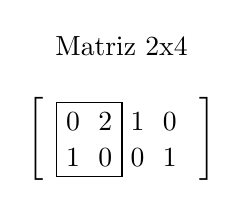
\begin{tikzpicture}[baseline=(M.center)]
 \matrix (M) [matrix of math nodes,left delimiter={[},right delimiter={]}] {
 0 & 2 & 1 & 0 \\
 1 & 0 & 0 & 1 \\
 };
 \draw (M-1-1.north west) rectangle (M-2-2.south east);
 \node[above=10pt of M.north] {Matriz 2x4};
\end{tikzpicture}
\hspace{0.8cm}\bigotimes\hspace{0.8cm}
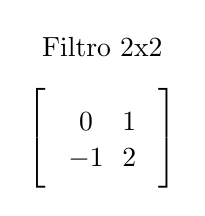
\begin{tikzpicture}[baseline=(M.center)]
 \matrix (M) [matrix of math nodes,left delimiter={[},right delimiter={]}] {
  0 & 1 \\
 -1 & 2 \\
 };
 \node[above=10pt of M.north] {Filtro 2x2};
\end{tikzpicture}
\hspace{0.8cm}=\hspace{0.8cm}
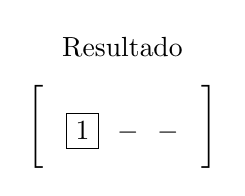
\begin{tikzpicture}[baseline=(M.center)]
 \matrix (M) [matrix of math nodes,left delimiter={[},right delimiter={]}] {
    \boxed{1} & - & - \\
 };
 \node[above=10pt of M.north] {Resultado};
\end{tikzpicture}
$$

$$
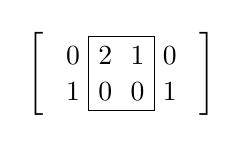
\begin{tikzpicture}[baseline=(M.center)]
 \matrix (M) [matrix of math nodes,left delimiter={[},right delimiter={]}] {
    0 & 2 & 1 & 0 \\
    1 & 0 & 0 & 1 \\
 };
 \draw (M-1-2.north west) rectangle (M-2-3.south east);
\end{tikzpicture}
\hspace{0.8cm}\bigotimes\hspace{0.8cm}
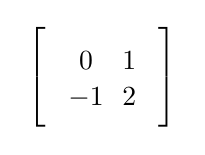
\begin{tikzpicture}[baseline=(M.center)]
 \matrix (M) [matrix of math nodes,left delimiter={[},right delimiter={]}] {
  0 & 1 \\
  -1 & 2 \\
 };
\end{tikzpicture}
\hspace{0.8cm}=\hspace{0.8cm}
\begin{bmatrix}
 1 & \boxed{1} & - \\
 \end{bmatrix}
$$

$$
\hspace{0.2cm}
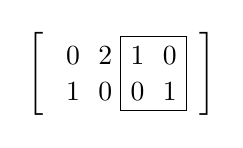
\begin{tikzpicture}[baseline=(M.center)]
 \matrix (M) [matrix of math nodes,left delimiter={[},right delimiter={]}] {
    0 & 2 & 1 & 0 \\
    1 & 0 & 0 & 1 \\
 };
 \draw (M-1-3.north west) rectangle (M-2-4.south east);
\end{tikzpicture}
\hspace{1cm}\bigotimes\hspace{0.9cm}
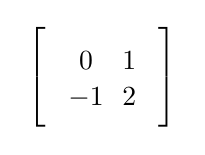
\begin{tikzpicture}[baseline=(M.center)]
 \matrix (M) [matrix of math nodes,left delimiter={[},right delimiter={]}] {
  0 & 1 \\
  -1 & 2 \\
 };
\end{tikzpicture}
\hspace{0.8cm}=\hspace{0.8cm}
\begin{bmatrix}
 1 & 1 &  \boxed{2} \\
 \end{bmatrix}
$$

\subsection*{Tamanho do passo e preenchimento}

O Tamanho do passo — ou stride — serve para especificar a distancia de pixels entre os passos da camada.  No exemplo acima esse parâmetro é definido como 1, por isso a matriz selecionada pula 1 pixel para direita entre os passos. Esse valor altera o tamanho da matriz resultante \cite{dp_overview}.

O preenchimento — ou padding — é uma técnica utilizada para manter o mesmo tamanho da entrada, adicionando bordas com zeros antes das operações da camada para ter como saída uma matriz do mesma dimensão da matriz original. Isso é usado devido a desvantagem em perder os detalhes nas bordas das imagens no processamento de uma camada \cite{dp_overview}.

\subsection*{Camada de agrupamento}

A camada de agrupamento — ou pooling — tem como tarefa primordial uma técnica para reduzir o tamanho do mapa de características, porém preservando os padrões mais relevantes. Dentre os recursos essenciais dessa camada estão o tamanho do agrupamento e a operação que será realizada. O maior problema dessa camada é pelo fato dela apenas identificar aonde essas características estão e não se tem ou não, \emph{i.e.}, dependendo de qual operação e a quantidade de camadas pode não ser possível guardar as principais características de forma integra causando uma redução no desempenho final da predição \cite{dp_overview}.

Existem vários tipos de agrupamento, os mais utilizados são: agrupamento máximo, agrupamento médio e agrupamento global médio que estão explicados abaixo em exemplos baseados em \citeonline{Alzubaidi2021}.

\subsubsection*{Agrupamento máximo}

É definido o resultado final com base no máximo encontrado pelo tamanho do agrupamento, exemplo a seguir usando um mapa de características com tamanho 4x4 e agrupamento de tamanho 2x2.

$$
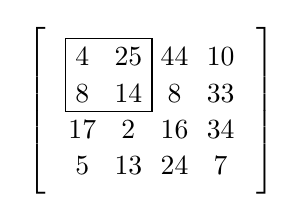
\begin{tikzpicture}[baseline=-0.5ex]
    \matrix (M) [matrix of math nodes,left delimiter={[},right delimiter={]}] {
        4 & 25 & 44 & 10\\
        8 & 14 & 8 & 33 \\
        17 & 2 & 16 & 34 \\
        5 & 13 & 24 & 7 \\
    };
    \draw (M-1-1.north west) rectangle (M-2-2.south east);
\end{tikzpicture}
= 
\begin{bmatrix}
	\boxed{25} & 44 \\
	17 & 34 \\
   \end{bmatrix}
$$

\subsubsection*{Agrupamento médio}

É definido o resultado final com base na média encontrada pelo tamanho do agrupamento, exemplo a seguir usando um mapa de características com tamanho 4x4 e agrupamento de tamanho 2x2.

$$
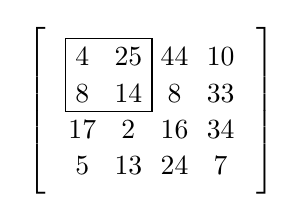
\begin{tikzpicture}[baseline=-0.5ex]
    \matrix (M) [matrix of math nodes,left delimiter={[},right delimiter={]}] {
        4 & 25 & 44 & 10\\
        8 & 14 & 8 & 33 \\
        17 & 2 & 16 & 34 \\
        5 & 13 & 24 & 7 \\
    };
    \draw (M-1-1.north west) rectangle (M-2-2.south east);
\end{tikzpicture}
= 
\begin{bmatrix}
	\boxed{12} & 23 \\
	9 & 20 \\
   \end{bmatrix}
$$

\subsubsection*{Agrupamento global médio}

É definido o resultado final com base na média geral do mapa o que sempre tem como saída uma matrix 1x1, exemplo a seguir usando um mapa de características com tamanho 4x4.

$$
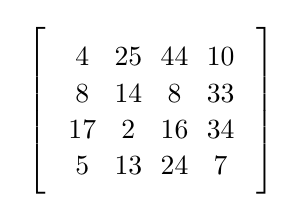
\begin{tikzpicture}[baseline=-0.5ex]
    \matrix (M) [matrix of math nodes,left delimiter={[},right delimiter={]}] {
        4 & 25 & 44 & 10\\
        8 & 14 & 8 & 33 \\
        17 & 2 & 16 & 34 \\
        5 & 13 & 24 & 7 \\
    };
\end{tikzpicture}
= 
\begin{bmatrix}
	16
   \end{bmatrix}
$$

\subsection*{Camada totalmente conectada}

A camada totalmente conectada geralmente é utilizada no final da arquitetura e cria a partir de cada neurônio uma ligação direta para cada etiqueta final. Isso torna essa camada extremamente pesada computacionalmente. O número de neurônios dessa camada é equivalente ao número de classes propostas. Além disso é quando chega nessa camada que a função de perda é calculada e se inicia a retropropagação \cite{Alzubaidi2021, computation11030052}.

\subsection*{Função de perda}
A função de perda é calculada na camada de saída e serve para mensurar o sucesso obtido comparando com fórmulas o resultado da arquitetura com o resultado real do conjunto de dados. O resultado dessa função irá ajudar na retropropagação, \emph{i.e.}, servirá para ajustar os pesos e viéses da conexão entre os neurônios para minimizar o erro. A seguir algumas funções de perda, pontuando que todo esse subtópico é baseado em 
\citeonline{Alzubaidi2021}.

\subsubsection*{Softmax ou entropia cruzada ou logarítmica}
Muito utilizada para medir a performace de uma rede neural convolucional principalmente quando o resultado final têm várias classes. Antes dessa função de perda é necessário usar a função de ativação softmax descrita na \cref{fig:grafico_softmax} pois precisa de uma saída dentro de uma distribuição de probabilidade. Sendo N o número de classes ou o número de neurônios na camada de saída.

$$H(p,y) = -\sum_{i=1}^N y_i \log(p_i)$$

\subsubsection*{Euclidiana ou erro quadrático médio}
Muito utilizada para problemas de regressão.

$$H(p,y) = \frac{1}{2N} \sum_{i=1}^N (p_i - y_i)^2$$

\subsubsection*{Hinge}
Muito utilizado para classificação binária.

$$H(p,y) = \sum_{i=1}^N max(0, m - (2y_i - 1) p_i)$$

\subsection*{Regularização}
Quando se monta uma arquitetura de redes neurais convolucional pode se chegar em três casos sendo eles: sobreajuste (overfit), subajuste (underfit) e balanceado (optimal). O sobreajuste é quando no treinamento o modelo acerta as classes porém nos testes não, isso mostra uma dificuldade em generalizar as características. Já o subajuste não consegue pontuar bem em nenhum caso mostrando que o conjunto de dados de treinamento está pequeno para detectar padrões. Por outro lado o balanceado é quando produz resultados bons tanto no conjunto de dados de treinamento quanto no de testes \cite{Alzubaidi2021, computation11030052}.

\begin{figure}[H]
	\caption{Gráficos mostrando subajuste, balanceado e sobreajuste respectivamente}
	\centering % para centralizarmos a figura
	\includegraphics[width=15cm]{figures/fittings.png} % leia abaixo
	\legend{Fonte: \citeonline{educative2022overfitting}}
	\label{fig:arquitetura_cnn}
\end{figure}

Segundo \citeonline{Alzubaidi2021} existem algumas alternativas para evitar o sobreajuste e o subajuste, dentre alguma estão:

\begin{itemize}
    \item Dropout: Muito utilizada para evitar sobreajuste pois está técnica irá desligar um neurônio aleatoriamente colocando a saída dele como zero no processo de treinamento e portanto forçara o modelo a aprender a indentificar características diferentes em outros neurônios possibilitando a generalização do modelo.
    \item Aumentar o tamanho do conjunto de dados: caso não seja possível criar ou encontrar um maior existem técnicas para aumentar artificialmente acrescentando pequenas mudanças nas imagens existentes, algumas são rotacionar, recortar e inverter horizontamente ou verticalmente.
\end{itemize}

\subsection*{Retropropagação}
De acordo com \citeonline{brilliant2023backpropagation} o algoritmo geral de retropropagação é:

\begin{enumerate}
    \item Propagação: calcular os pares de entrada-saída $(\overrightarrow{x_d}, y_d)$ — $\overrightarrow{x_d}$ é o vetor de entrada e $y_d$ a saída verdadeira — e guardar os resultados $\hat{y_d}$ — a saída encontrada no treinamento —, $a_j^k$, $o_j^k$ para cada neurônio $j$ na camada $k$, indo da camada de entrada para camada de saída.
    
    \item Retropropagação: Calcular os pares de entrada-saída $(\overrightarrow{x_d}, y_d)$, chegando na fórmula $\frac{\partial{E_d}}{\partial{w_{ij}^k}}$ que é a derivada parcial do erro total. Na representação $E_d$ é a função de perda e $w_{ij}^k$ é o peso  conectado em um neurônio de $k - 1$. Outra forma de representar é $\delta_j^k o_i^{k - 1}$ e suas variáveis são: $\delta_j^k$ representa o erro do neurônio e $o_i^{k - 1}$ representa a saída do neurônio na camada $k -1$. Essa técnica começa na camada de saída e propaga até a última camada escondida.
    
    $$ \frac{\partial{E_d}}{\partial{w_{ij}^k}} = \delta_j^k o_i^{k - 1} $$
    
    \item Combinar gradientes individuais: Uma média simples é feita com todos resultados de $\frac{\partial{E_d}}{\partial{w_{ij}^k}}$ formando assim o gradiente total representado como $\frac{\partial{E(X, \theta)}}{\partial{w_{ij}^k}}$.
    
    $$ \frac{\partial{E(X,\theta)}}{\partial{w_{ij}^k}} = \frac{1}{N} \sum_{d=1}^{N} \frac{\partial{E_d}}{\partial{w_{ij}^k}} $$
    \item Atualiza os pesos: usando $\alpha$ como taxa de aprendizado e o gradiente total $\frac{\partial{E(X, \theta)}}{\partial{w_{ij}^k}}$ temos a seguinte equação.
    
    $$ \Delta w_{ij}^k = -\alpha \frac{\partial{E(X,\theta)}}{\partial{w_{ij}^k}} $$
\end{enumerate}

Observação: basta trocar $w_{ij}^k$ para $b_{ij}^k$ — trocar o peso pelo viés — em todo algoritmo para ajustar o viés do modelo com a tecnica de retropropagação.

\subsection*{Melhorar performace}

Com base em testes de aplicações existem algumas maneiras de melhorar a qualidade do resultado final do modelo sendo elas \cite{Alzubaidi2021}:

\begin{itemize}
    \item Aumentar o conjunto de dados
    \item Aumentar o tempo de treinamento
    \item Aumentar a profundidade ou largura da arquitetura
    \item Regularizar o modelo
    \item Ajustar os hiperparâmetros
\end{itemize}
    

\subsubsubsection*{Segmentação}
\label{sec:segmentacao}

O estudo de segmentação semântica dentro da área de redes neurais convolucionais têm três principais nichos, sendo eles: segmentação semântica que é a classificação por pixel, a segmentação de instância que atribui um id para cada objeto encontrado de uma classe, e a segmentação panóptica que junta as duas anteriores para criar uma imagem semelhante a saída de segmentação semântica porém separando objetos de mesma classe sendo essa a mais recente e completa, a diferença entre esses três tipos está ilustrado na \cref{fig:segentacoes} \space\cite{dp_semantic_segmantation, lapix}.

\begin{figure}[ht]
	\caption{Tipos de segmentação em redes neurais convolucionais}
	\centering % para centralizarmos a figura
	\includegraphics[width=10cm]{figures/segmantations.png} % leia abaixo
	\legend{Fonte: \citeonline{kirillov2019panoptic}}
	\label{fig:segentacoes}
\end{figure}

\subsubsubsection*{Segmentação semântica}

A segmentação semântica começou a ter resultados satisfatórios a partir de redes totalmente convolucionais, com o objetivo de segmentar imagens classificando pixels, esse modelo descarta a camada totalmente conectada pois a saída deverá ser uma imagem e não uma classificação — isso a torna mais rápida para treinar do que as redes neurais convolucionais —, logo usa camadas deconvolucionais para transformar a matriz de características em uma imagem de qualquer dimensão na saída. A RTC criou a arquitetura chamada de salto (ou conexões) que serve para evitar perdas em camadas de agrupamento criando conexões entre camadas não consecutivas — geralmente entre camadas convolucionais e deconvolucionais — como apresentado na \cref{fig:rtc}, a arquitetura de salto evoluiu para arquitetura codificador-decodificador.
\begin{figure}[ht]
	\caption{Exemplo de arquitetura de rede totalmente convolucional}
	\centering % para centralizarmos a figura
	\includegraphics[width=10cm]{figures/redes_totalmente_convolucionais.png} % leia abaixo
	\legend{Fonte: \citeonline{dp_semantic_segmantation}}
	\label{fig:rtc}
\end{figure}

A arquitetura codificador-decodificador — ou Encoder-Decoder —, é separada em dois passos: o primeiro para convergir no mapa de características — chamado de codificador — e o segundo para reverter — chamado de decodificador — as camadas de agrupamento para aumentar a dimensão da saída, usando camadas deconvolucionais e de desagrupamento. Outra característica importante é a conexão entre camadas de mesmo nível, como por exemplo a arquitetura UNet, que foi a primeira a implementar o padrão Codificador-Decodificador. Na \cref{fig:unet} pode-se observar que tem formato da letra U, sendo a descida a parte de codificação e subida decodificação \space\cite{dp_semantic_segmantation, lapix, unetArq}.

\begin{figure}[ht]
	\caption{Arquitetura codificador-decodificador UNet}
	\centering % para centralizarmos a figura
	\includegraphics[width=10cm]{figures/unet.png} % leia abaixo
	\legend{Fonte: \citeonline{unetArq}}
	\label{fig:unet}
\end{figure}

\subsubsubsection*{Segmentação de instância}

Outro problema dentro da área de visão computacional é a detecção de objetos, a primeira solução foi com Características de regiões com RNC — Regions with CNN features (R-CNN) — que se resume em dividir a imagem de entrada em regiões de interesse e nessas regiões aplicar uma RNC. A arquitetura que seleciona essas regiões é chamada de Rede de Proposta de Região (RPR) — ou Region Proposal Network (RPN) — o que auxilia na detecção por caixas delimitadoras. Essa ideia inicial foi estendida para segmentação de instância criando também máscara nos objetos, como por exemplo a arquitetura Mask R-CNN \space\cite{dp_semantic_segmantation, lapix}.

A arquitetura Mask R-CNN é derivado do Fast R-CNN — aprimoramento do R-CNN aplicando conceito RoIPool para classificar — onde há uma segmentação de máscara em cada RoI — ou Região de interesse — paralela com a classificação da caixa delimitadora. A máscara é classificada com uma pequena RTC em cada RoI. Além de ter uma pequena melhoria na RoIPool, pois havia um problema de alinhamento nas localizações espaciais exatas, essa camada é chamada de RoIAlign \space\cite{maskRCNN}.

\subsubsubsection*{Segmentação panóptica}

Um problema encontrado na segmentação semântica é que objetos de mesma classe não são separados como na segmentação de instância, logo surgiu uma ideia para criar uma solução usando as duas técnicas. Esse conceito surgiu do trabalho \citeonline{kirillov2019panoptic} e consiste na definição geral da ideia, uma métrica — que será explicada posteriormente — unificada para classificar os resultados do modelo além de fazer a distinção entre coisas — ou stuff — que não são contáveis, como o céu e os objetos — ou things — que são contáveis como carros, pessoas, etc.
Os principais conjunto de dados para tarefa panóptica são COCO-Panoptic, Cityscapes, Mapillary Vistas, ADE20K, e Indian Driving Dataset. Cada conjunto de dados possui diversas classes para o modelo aprender \space\cite{v7labs2022panoptic}.

\subsubsubsection*{Métricas e técnicas}
\label{sec:metricas_tecnicas}

No ramo de segmentação existem diversas métricas que podem ser usadas, dentre elas algumas serão destacas nesta monografia a seguir:

\subsubsubsection*{Classificação de conjuntos}
\label{sec:classificacao_conjuntos}

A classificação de conjuntos é uma técnica para criar relações entre a imagem de predição e a imagem do conjunto de dados. Ela se divide em quatro conjuntos sendo eles: Positivo Verdadeiro — ou True Positive(TP) —
% sendo o requisito ter uma intersecção significativa entre classes iguais, \emph{i.e.}, IoU > 0.5
, Negativo Verdadeiro — ou True Negative(TN) —, Falso Positivo — ou False Positive(FP) — quando um objeto não é correspondido na imagem de predição e por fim o Falso Negativo — ou False Negatives(FN) — quando um objeto não é correspondido na imagem do conjunto de dados. Essa técnica pode ser usada em modelos de classificação binária usando uma matriz de confusão mas na área de segmentação costuma-se contar os pixeis e sua representação visual pode-se observar na \cref{fig:conjuntos} \space\cite{kirillov2019panoptic, Wang2020}.
\begin{figure}[ht]
	\caption{Exemplo da classificação dos conjuntos usados nas métricas de segmentação}
	\centering % para centralizarmos a figura
	\includegraphics[width=15cm]{figures/pan_metric.png} % leia abaixo
	\legend{Fonte: \citeonline{slidesKirillov} editado}
	\label{fig:conjuntos}
\end{figure}


\subsubsubsection*{F1 Score}

O F1 Score é uma métrica que pode ser utilizada para calcular a eficiência de modelos de segmentação de instância,  baseando-se em encontrar uma relação entre a área das classes da imagem de saída com as classes na imagem do conjunto de dados porém diminuindo o peso dos erros. Varia de 0 a 1 sendo 1 com maior eficiência. Segue a exemplificação da \cref{eq:f1} \space\cite{Chicco2020}:

\begin{equation}
	\label{eq:f1}
	F1\ Score = \frac{\text{TP}}{(TP + \frac{FP}{2} + \frac{FN}{2} )}
\end{equation}

\subsubsubsection*{Coeficiente de correlação de Matthews}

O coeficiente de correlação de Matthews — ou Matthews Correlation Coefficient (Mcc) —  é uma métrica que pode ser utilizada para mensurar a eficiência de modelos de segmentação,  baseando-se no coeficiente de correlação de Pearson. Varia de -1 a 1 sendo 1 com maior correlação, 0 inconclusivo e -1 sem correlação. Segue a exemplificação da \cref{eq:mcc} \space\cite{Chicco2020, confusion_matrix_calculator}:

\begin{equation}
	\label{eq:mcc}
	Mcc = \frac{\text{TP}\cdot\text{TN}-\text{FP}\cdot\text{FN}}{\sqrt{ (\text{TP}+\text{FP})\cdot(\text{TP}+\text{FN})\cdot(\text{TN}+\text{FP})\cdot(\text{TN}+\text{FN}) }}
\end{equation}

\subsubsubsection*{Taxa de descoberta falsa}

A taxa de descoberta falsa — ou False Discovery Rate (FDR) — é uma métrica utilizada para calcular o erro obtido na imagem de predição,  baseando-se em encontrar uma relação entre ao erro obtido, divido pelo erro mais acerto esperado. Varia de 0 a 1 sendo 1 o pior caso e 0 o melhor. Segue a exemplificação da \cref{eq:fdr} \space\cite{confusion_matrix_calculator}:

\begin{equation}
	\label{eq:fdr}
	Fdr = \frac{FP}{FP + TP}
\end{equation}


\subsubsubsection*{Taxa de Falso Negativo}

A taxa de falso negativo — ou False Negative Rate (FNR) — é uma métrica utilizada para calcular o erro obtido na imagem verdade,  baseando-se em encontrar uma relação entre ao erro obtido, divido pelo erro mais acerto esperado. Varia de 0 a 1 sendo 1 o pior caso e 0 o melhor. Segue a exemplificação da \cref{eq:fnr} \space\cite{confusion_matrix_calculator}:

\begin{equation}
	\label{eq:fnr}
	Fnr = \frac{FN}{FN + TP}
\end{equation}

\subsubsubsection*{Acurácia}

A acurácia — ou Accuracy (Acc) — é uma métrica utilizada para calcular a eficiência de modelos de segmentação semântica,  baseando-se em encontrar uma relação entre a área das classes da imagem de saída com as classes na imagem do conjunto de dados para todos conjuntos. Varia de 0 a 1 sendo 1 com maior eficiência. Segue a exemplificação da \cref{eq:acc} \space\cite{Chicco2020}:

\begin{equation}
	\label{eq:acc}
	Acc = \frac{\text{TP + TN}}{\text{(TP + TN + FP + FN)}}
\end{equation}

\subsubsubsection*{União sobre intersecção}

A união sobre intersecção — Intersection over Union (IoU) — ou índice de Jaccard é uma métrica muito utilizada para calcular a eficiência de modelos de segmentação, ela se baseia em encontrar uma relação entre a área das classes da imagem de saída com as classes na imagem do conjunto de dados para qualquer valor positivo, isto é, desconsiderando o conjunto positivo falso. Varia de 0 a 1 sendo 1 com maior eficiência. Segue a exemplificação da \cref{eq:iou} \space\cite{iou_metric_link}:

\begin{equation}
	\label{eq:iou}
	IoU = \frac{\text{TP}}{\text{(TP + FP + FN)}}
\end{equation}

\subsubsubsection*{Qualidade panóptica}

A qualidade panóptica — ou Panoptic Quality (PQ) — foi definido pela primeira vez no artigo \citeonline{kirillov2019panoptic}, e se resume na fórmula:

\begin{equation}
\label{eq:pq_metric}
PQ = \frac{\sum_{(p,g)\in TP}IoU(p,g)}{ |TP| + \frac{1}{2}|FP| + \frac{1}{2}|FN|}
\end{equation}

Multiplicando a \cref{eq:pq_metric} por $\frac{|TP|}{|TP|}$ tem-se:

\begin{equation}
	\label[]{eq:pq_metric_mult}
	PQ = \underbrace{\frac{\sum_{(p,g)\in TP}IoU(p,g)}{|TP|}}_{\text{Segmentation Quality (SQ)}}
	\times
	\underbrace{\frac{|TP|}{|TP| + \frac{1}{2}|FP| + \frac{1}{2}|FN|}}_{\text{Recognition Quality (RQ)}}
\end{equation}

Portanto pode-se concluir que PQ é apenas uma simplificação para uma fórmula que contém uma relação entre métricas de segmentação semântica e de instância.

Com base no subtópico \hyperref[sec:segmentacao]{Segmentação} percebe-se que a segmentação panóptica é a mais completa e por efeito de estudos será utilizado o mesmo para concluir o trabalho. Como nesse nicho existem várias alternativas será utilizado a métrica demonstrada na \cref{eq:pq_metric} para analisar resultados e selecionar o modelo.

\subsubsubsection*{Resultados de modelos do nicho de segmentação panóptica}

Os resultados são de uma competição em aberto criada pela Cityscapes Dataset, essa competição tem várias modalidades e esses são referentes ao nicho de segmentação panóptica utilizando a métrica PQ na classe de pessoas. A exibição dos resultados contendo a métrica PQ que classifica pessoas com os quinze melhores modelo encontra-se na \cref{tab:resultados-cityscapes} \space\cite{datasetResults}.
\begin{table}[h]
	\centering
	\caption{Top 15 modelos que melhor classificam pessoas com métrica P em segmentação panóptica}
	\label{tab:resultados-cityscapes}
	\begin{tabular}{|l|c|}
	  \hline
	  Nome do modelo & PQ (\%) \\
	  \hline
	  EfficientPS [Mapillary Vistas] & 61,6 \\
	  EfficientPS [Cityscapes-fine] & 60,9 \\
	  Panoptic-DeepLab w/ SWideRNet [Mapillary Vistas + Pseudo-labels] & 60,6 \\
	  hri\_panoptic & 60,6 \\
	  Naive-Student (iterative semi-supervised learning with Panoptic-DeepLab) & 60,2 \\
	  Panoptic-DeepLab w/ SWideRNet [Mapillary Vistas] & 59,8 \\
	  iFLYTEK-CV & 59,2 \\
	  Panoptic-DeepLab [Mapillary Vistas] & 58,5 \\
	  Panoptic-DeepLab w/ SWideRNet [Cityscapes-fine] & 58,4 \\
	  Seamless Scene Segmentation & 57,7 \\
	  Axial-DeepLab-XL [Mapillary Vistas] & 57,2 \\
	  Unifying Training and Inference for Panoptic Segmentation [COCO] & 56,5 \\
	  kMaX-DeepLab [Cityscapes-fine] & 56 \\
	  Axial-DeepLab-L [Mapillary Vistas] & 55,9 \\
	  TASCNet-enhanced & 55,2 \\
	  \hline
	\end{tabular}
  \end{table}





\subsection{Visão computacional}
A visão computacional avança cada vez mais, aproximando os computadores da capacidade visual humana.Segundo Horst Haußecker e Bernd Jähne no livro "Computer Vision and Applications" \cite{comp_vision_and_applications}, a visão computacional é uma área da computação que se dedica à interpretação de imagens por meio de algoritmos e técnicas de processamento de imagens. Essa área abrange a aquisição, processamento e análise de imagens, com o objetivo de extrair informações úteis para resolver problemas específicos.

A visão é um elemento crucial para capacitar a inteligência artificial a realizar diversas tarefas. A fim de replicar a visão humana, é necessário que as máquinas sejam capazes de adquirir, processar, analisar e compreender imagens. \cite{como_funciona_visao_computacional}

Na \cref{fig:comp_vision} podemos ver uma analogia entre a forma como uma imagem é processada pelo cérebro humano e a forma como é processada por um sistema computacional.

\begin{figure}[!ht]
	\centering
	\includegraphics[width=0.6\textwidth]{figures/content_Human_Vision.png}
	\caption{Comparação entre a forma de como o cérebro humano e um computador processam informações \cite{content_Human_Vision}.}
	\label{fig:comp_vision}
\end{figure}	

\subsubsection{Pré-processamento de Imagens}

\subsubsection{Detectação de objetos}

\subsubsection{Segmentação de imagem}

\subsection{Algoritmos de segmentação}

\section{Geração procedural}
\subsection{Diagrama de Voronoi}

O diagrama de Voronoi é gerado a partir das distancias euclidianas entre os vizinhos mais próximos de um conjunto de pontos do plano\space
\cite{diagrama_de_voronoi:_uma_exploracao_nas_distancias_euclidiana_e_do_taxi}. Esse diagrama possui uma gama de utilizações, por exemplo, estudar epidemias, encontrar o 
ponto mais próximo, calcular a precipitação de uma área, estudar os padrões de crescimento das florestas, etc,\space\cite{poligonos_de_thiessen_ou_voronoi}. 

Seja um conjunto de índices $I_n = \{1, 2, 3, ..., n\}$ e $A = \{p_1, p_2, ..., p_n\} \subset \mathbb{R}^2$ um conjunto de pontos onde $2 \leq n < \infty$, definimos como região de Voronoi o conjunto de pontos associado a $p_i$, onde d é a distancia euclidiana

$$V(p_i) = \{p|d(p_i,p) \leq d(p_i,p);i \neq j, i, j \in I_n\},$$

temos o conjunto formado por essas regiões sendo $V(A) = {V(1), V(2), V(3), ..., V(n)}$ \cite{rodrigues_diagrama_2019}.

Na figura \cref{fig:diagrama_voronoi} podemos ver a relação do conjuntos de pontos com o diagrama de Voronoi.
\begin{figure}[H]
	\centering
	\includegraphics[width=0.8\textwidth]{figures/diagrama_de_voronoi.png}
	\caption{Diagrama de Voronoi \cite{thomazthz_diagrama_2014}.}	
	\label{fig:diagrama_voronoi}
\end{figure}



\section{Trabalhos relacionados}

Esta seção destina-se a análise e discussão da metodologia e dos resultados prospostos por \citeonline{geracao_procedural_jogos_2d,kirillov2019panoptic}. 

\subsection*{Geração Procedural de Mapas para Jogos 2D}

No trabalho \citeonline{geracao_procedural_jogos_2d}, é apresentado uma solução simples para criar mapas de cavernas, calabouços e ilhas para jogos 2D. O algoritmo foi dividido em três partes sendo elas: geração recursiva de terrenos, validação de tamanho e correção da coesão. Os autores concluíram que não existe literatura sobre geração procedural de salas diversas e corredores distintos como o algoritmo proposto. Sugerem duas possibilidades para trabalhos futuros sendo elas: usar algoritmos genéticos para mensurar a qualidade dos mapas gerados e promover pela seleção natural e a outra possibilidade é mesclar o algoritmo proposto com técnicas de geração de salas interligadas por corredores, de forma a possibilitar a criação de mapas com algumas salas pré-definidas inseridas em um mapa aberto contínuo.

\subsection*{Panoptic Segmentation}

No trabalho \citeonline{kirillov2019panoptic} é definido a ideia geral de segmentação panóptica além de definir conceitos importantes como coisas e objetos e a métrica unificada para medir o desempenho de modelos dessa área. Também é feito alguns testes comparando resultados humanos com um modelo simples proposto com eles combinando PSPNet e Mask R-CNN usando a métrica de qualidade panóptica definida por eles. Os resultados mostraram a superioridade humana na segmentação panóptica em três conjuntos de dados diferentes, sendo eles: Cityscapes, ADE20k e Vistas, as métricas usadas foram qualidade panóptica, qualidade semântica, qualidade de reconhecimento, qualidade panóptica
 de coisas e qualidade panóptica de objetos. O melhor resultado para a máquina em comparação com o humano foi no conjunto de dados Cityscapes avaliando a qualidade semântica, sendo 84,1 para o humano e 80,9 para máquina. O pior resultado para a máquina em relação ao humano foi no conjunto de dados ADE20k na qualidade panóptica de coisas, sendo 71,0 para os humanos e 24,5 para a máquina.

 \subsection*{Polygonal Map Generation for Games}

 No artigo de \citeonline{amitp2010} é apresentado toda uma jornada de desenvolvimento de um algoritmo de geração procedural de conteúdo, é mostrando as técnicas para gerar o mapa com o diagrama de Voronoi, gerar os rios e biomas utilizando as camadas de elevação e umidade do polígono e a aplicando isso no diagrama de Whittaker para definir o bioma do polígono. Também é apresentado uma técnica para adicionar ruídos nas arestas dos políginos fazendo com que o mapa se torne mais orgânico e realista.

\chapter{Desenvolvimento}


% ----------------------------------------------------------
% Finaliza a parte no bookmark do PDF
% para que se inicie o bookmark na raiz
% e adiciona espaço de parte no Sumário
% ----------------------------------------------------------
%\phantompart

% ---
% Conclusão (outro exemplo de capítulo sem numeração e presente no sumário)
% ---
\chapter*[Conclusão]{Conclusão}
\addcontentsline{toc}{chapter}{Conclusão}
% ---

\lipsum[31-33]

% ----------------------------------------------------------
% ELEMENTOS PÓS-TEXTUAIS
% ----------------------------------------------------------
\postextual
% ----------------------------------------------------------

% ----------------------------------------------------------
% Referências bibliográficas
% ----------------------------------------------------------
\bibliography{references}

% ----------------------------------------------------------
% Glossário
% ----------------------------------------------------------
%
% Consulte o manual da classe abntex2 para orientações sobre o glossário.
%
%\glossary

% ----------------------------------------------------------
% Apêndices
% ----------------------------------------------------------

% ---
% Inicia os apêndices
% ---
% \begin{apendicesenv}

% % Imprime uma página indicando o início dos apêndices
% \partapendices

% % ----------------------------------------------------------
% \chapter{Quisque libero justo}
% % ----------------------------------------------------------

% \lipsum[50]

% % ----------------------------------------------------------
% \chapter{Nullam elementum urna vel imperdiet sodales elit ipsum pharetra ligula
% ac pretium ante justo a nulla curabitur tristique arcu eu metus}
% % ----------------------------------------------------------
% \lipsum[55-57]

% \end{apendicesenv}
% ---


% ----------------------------------------------------------
% Anexos
% ----------------------------------------------------------

% ---
% Inicia os anexos
% ---
% \begin{anexosenv}

% % Imprime uma página indicando o início dos anexos
% \partanexos

% % ---
% \chapter{Morbi ultrices rutrum lorem.}
% % ---
% \lipsum[30]

% % ---
% \chapter{Cras non urna sed feugiat cum sociis natoque penatibus et magnis dis
% parturient montes nascetur ridiculus mus}
% % ---

% \lipsum[31]

% % ---
% \chapter{Fusce facilisis lacinia dui}
% % ---

% \lipsum[32]

% \end{anexosenv}

%---------------------------------------------------------------------
% INDICE REMISSIVO
%---------------------------------------------------------------------
%\phantompart
\printindex
%---------------------------------------------------------------------

\end{document}